\section{Методы обнаружения сигналов}
\label{sec:theory}

\newcommand{\AR}{\mathit{AR}}
\newcommand{\MA}{\mathit{MA}}
\newcommand{\ARMA}{\mathit{ARMA}}


\subsection{Общие сведения}

Обнаружение сигналов является фундаментальной задачей радиосвязи. Потребность в этом возникает в большинстве сценариев использования радиосредств, причем, каждая сфера применения определяет эту проблему по-своему. Пользовательским радиоприемникам нужно сканировать заданный диапазон на наличие наиболее мощных сигналов, которые достаточно сильно выделяются на общем фоне и непрерывны во времени. В служебной связи задача осложняется тем, что зачастую канал можно обнаружить только во время его использования. При дальней связи и связи в неблагоприятных условиях полоса частот известна заранее, но мощность сигнала меньше мощности шума, тогда обнаружить его означает подобрать подходящую модель, чтобы компенсировать помехи и извлечь полезную информацию. В сфере радиоразведки ведется постоянная гонка вооружений и данная проблема актуальна всегда.

Такое многообразие задач, имеющих общее название "<обнаружение сигналов">, очевидно, не может быть охвачено небольшим набором методов. Тем не менее, в их решении есть общая основа  --- представление сигнала. Радиоволна имеет вполне определенные физические характеристики, которые исследователь может представить в любой удобной для него форме.
Наиболее интуитивное их выражение --- это последовательность мгновенных уровней сигнала во времени. Оно полезно тем, что существует много методов для работы с временными рядами. Таким образом можно использовать достижения других областей науки и привносить в них свои новшества. Такой подход называется представлением сигнала во временном домене.
В этой форме, однако, не очевидно, как энергия волн распределена по частотам. А это свойство очень полезно, так как нас интересует, на каких частотах наблюдается активность. Поэтому, широкое применение нашел альтернативный подход --- представление сигнала в частотном домене. Оно не привносит новой информации, а является альтернативной формой записи параметров радиоволн. Переход от одного представления к другому осуществляется через прямое и обратное преобразование Фурье, о котором более подробно будет рассказано ниже.

Эти представления лежат в основе двух семейств методов: анализа временных рядов и спектрального анализа. Они решают разные задачи и дополняют друг друга.


\subsection{Авторегрессионная модель}

Авторегрессионная модель (Autoregressive model, $\AR$) --- это математическая модель случайного процесса, основывающаяся на предположении, что последующее значение последовательности линейно зависит от предыдущих (\autoref{eq:theory:ar}).

\begin{equation}
  \label{eq:theory:ar}
  X_t = \sum_{i=1}^p \phi_i X_{t-i} + \varepsilon_t
\end{equation}
\begin{explanation}
\item[где] $\phi_1, \dotsc, \phi_p$ --- параметры модели;
\item $\varepsilon_t$ --- шум.
\end{explanation}

Это достаточно простая конструкция, которая, впрочем, демонстрирует неплохие результаты и применяется как составная часть более сложных моделей.
Ее основные достоинства --- невысокая вычислительная сложность и возможность применения к любому временному ряду без его анализа. Так можно получать базовое качество оценки параметров ряда и использовать его для получения предварительных выводов.
Недостатки вытекают из простоты --- неспособность уловить сложные закономерности и неустойчивость к шуму.


Настройка авторегрессии заключается в подборе ее параметров. Это делается с помощью метода наименьших квадратов. Количество параметров называется порядком модели и записывается $\mathit{\AR}(n)$. Порядок подбирается вручную или методами выбора модели (AIC, BIC и другими). Он не должен быть слишком большим --- в этом случае невязка с данными, используемыми для настройки будет мала, а на новых сильно возрастет. Эта проблема известна как переобучение, то есть излишняя подстройка под обучающие данные, в результате чего страдает обобщающая способность модели.

Теоретически $\AR$ обоснована только для случайных процессов, обладающих свойством слабой стационарности, то есть математическое ожидание не изменяется во времени и функция автоковариации постоянна для сдвига $k$:

\begin{equation}
  \begin{split}
    E[X_t] & = const \\
    cov(X_{t_1}, X_{t_1-k}) & = cov(X_{t_2}, X_{t_2-k})
  \end{split}
\end{equation}

Это утверждение неверно применительно к радиосигналам, поэтому авторегрессионная модель в реальных ситуациях обладает слабой предсказательной силой, но по ее поведению все-равно можно сделать некоторые выводы о природе случайного процесса. Например, наблюдая за значениями невязки модельных и реальных данных можно заметить разладки в СП --- невязка резко возрастет.

Тем не менее, на очищенных от шума данных авторегрессия работает неплохо. $\AR(2)$ достаточно хорошо приближает модельный FM сигнал (\autoref{fig:theory:ar_pred_next}). Визуально отличия заметны только при детальном рассмотрении. Это можно объяснить гладкой формой синусоиды: каждое следующее значение не сильно отклоняется от предыдущих. При добавлении шума результат становится значительно хуже.

\begin{figure}[h]
  \centering
  \begin{subfigure}{0.45\textwidth}
    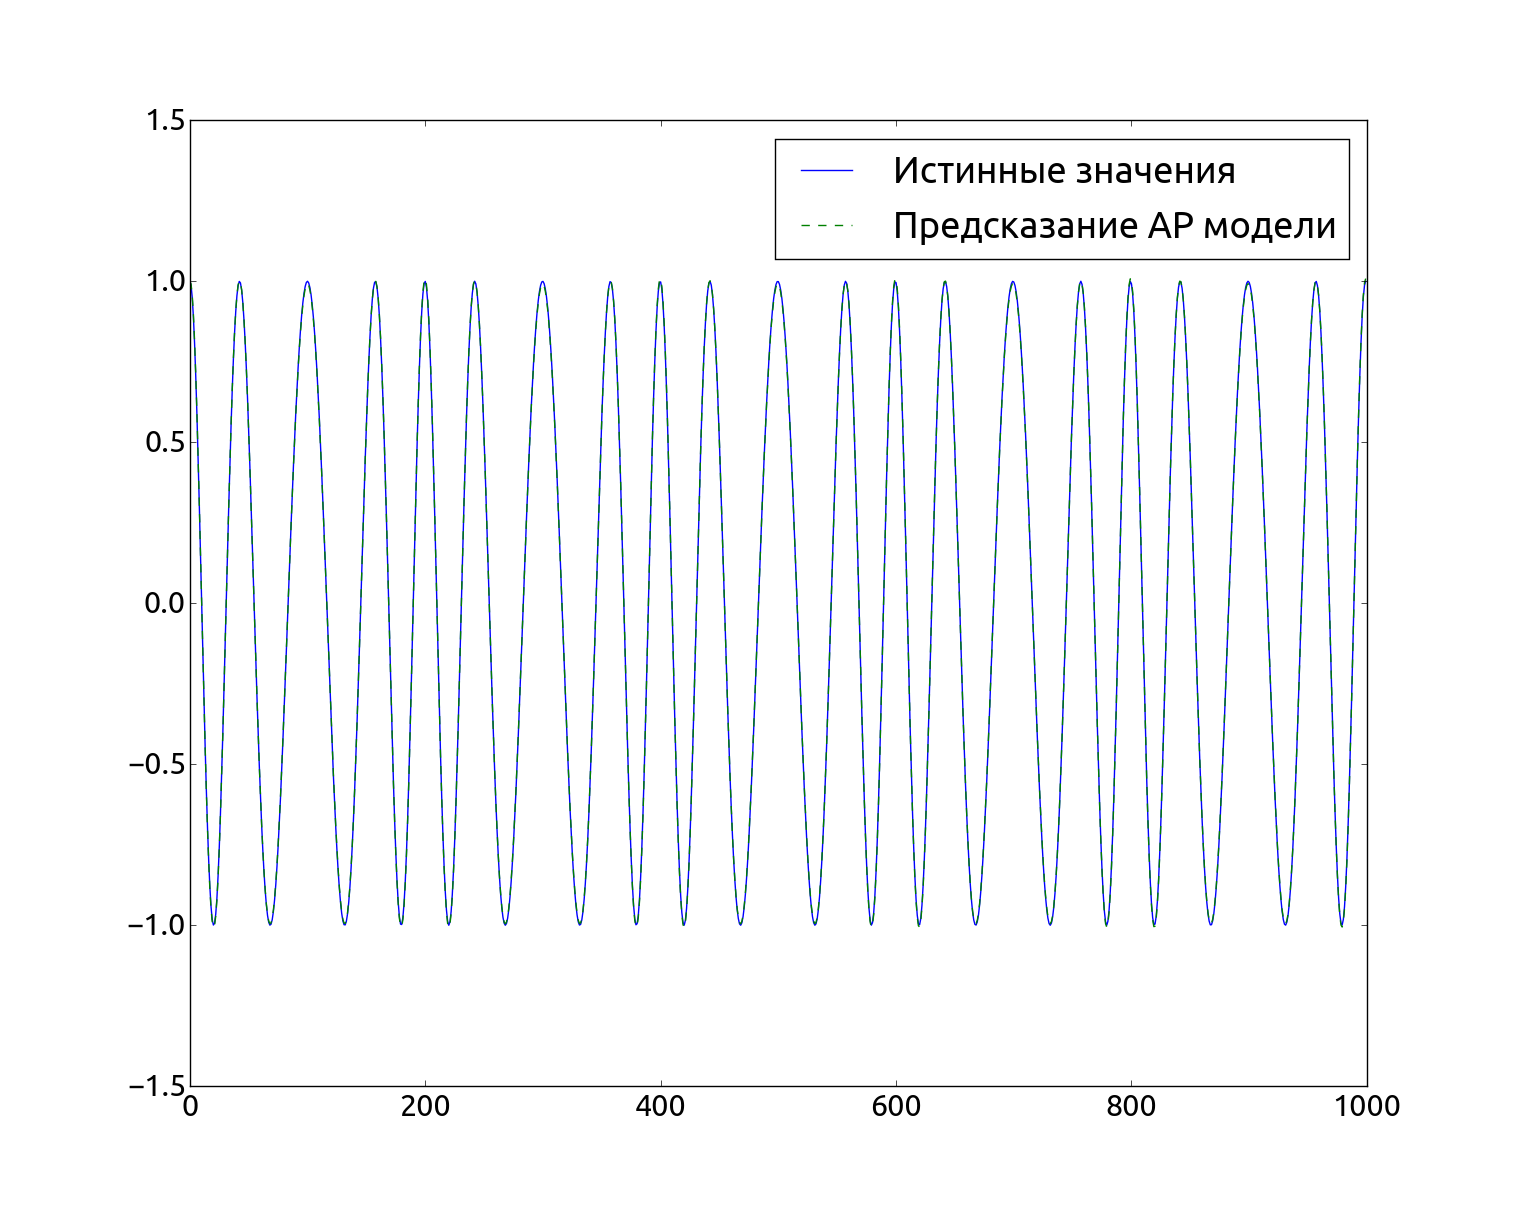
\includegraphics[width=\textwidth]{theory/ar_pred_next}
    \caption{}
    \label{fig:theory:ar_pred_next_whole}
  \end{subfigure}
  \begin{subfigure}{0.45\textwidth}
    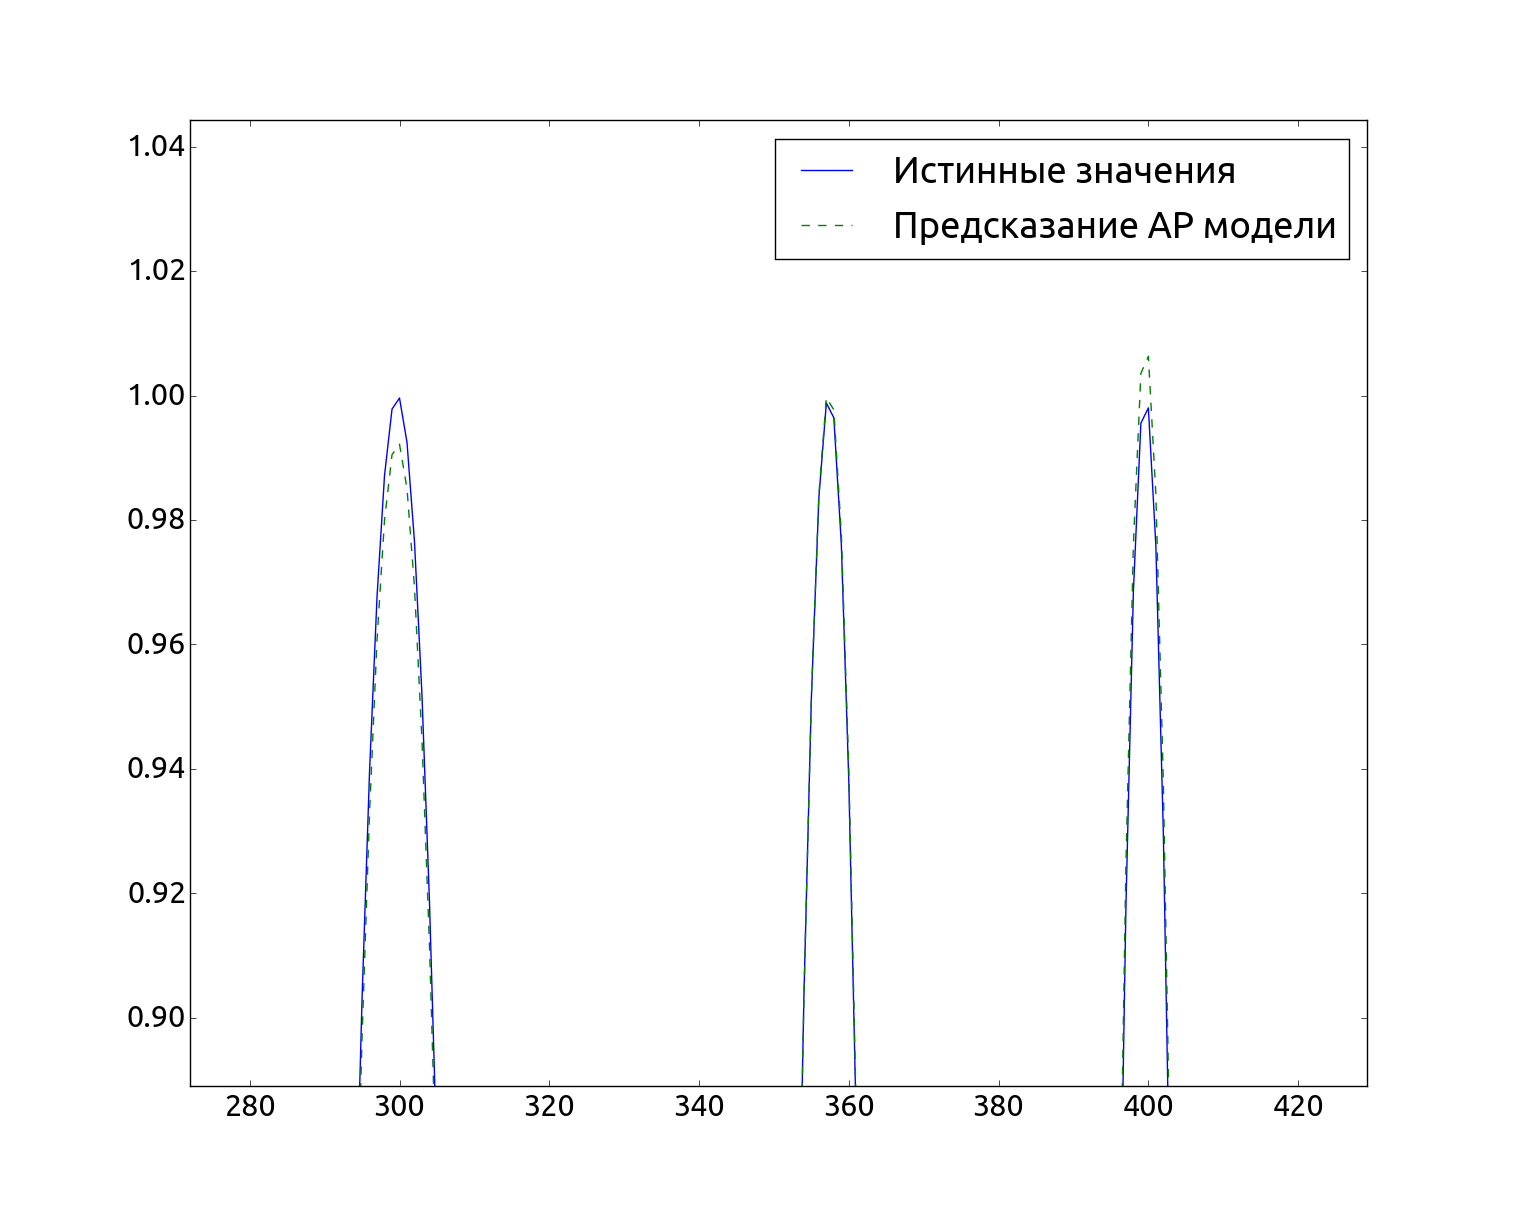
\includegraphics[width=\textwidth]{theory/ar_pred_next_zoomed}
    \caption{}
    \label{fig:theory:ar_pred_next_zoomed}
  \end{subfigure}
  \caption{Предсказания $\AR$ модели на основе реальных данных (\subref{fig:theory:ar_pred_next_whole}). Увеличенный участок графика (\subref{fig:theory:ar_pred_next_zoomed}).}
  \label{fig:theory:ar_pred_next}
\end{figure}

Чтобы построить этот график, были сгенерированы два временных ряда. Оба представляют собой частотно модулированную синусоиду. На первом была настроена $\AR(2)$, а второй использовался для контроля качества. Из него выбирались два последовательных элемента, и модель на их основе предсказывала следующий. Так был составлен ряд предсказаний модели. Как видно, она достаточно хорошо подстроилась под параметры сигнала. Ошибки можно заметить, если увеличить области перегибов синусоиды: сложно угадать точный угол при изменяющейся частоте.

Интересный эффект можно получить, если строить регрессию на ранее предсказанных данных. Ошибка модели накапливается и усиливается со временем, из-за чего сигнал обычно либо угасает, либо устремляется в бесконечность. Поэтому в расчетах стоит использовать только несколько ближайших предсказанных значений. Зато, при появлении новых наблюдений реальных значений не требуется перестраивать модель, ее параметры действительны, если описываемый случайный процесс не изменил своих параметров.

\begin{figure}[h]
  \centering
  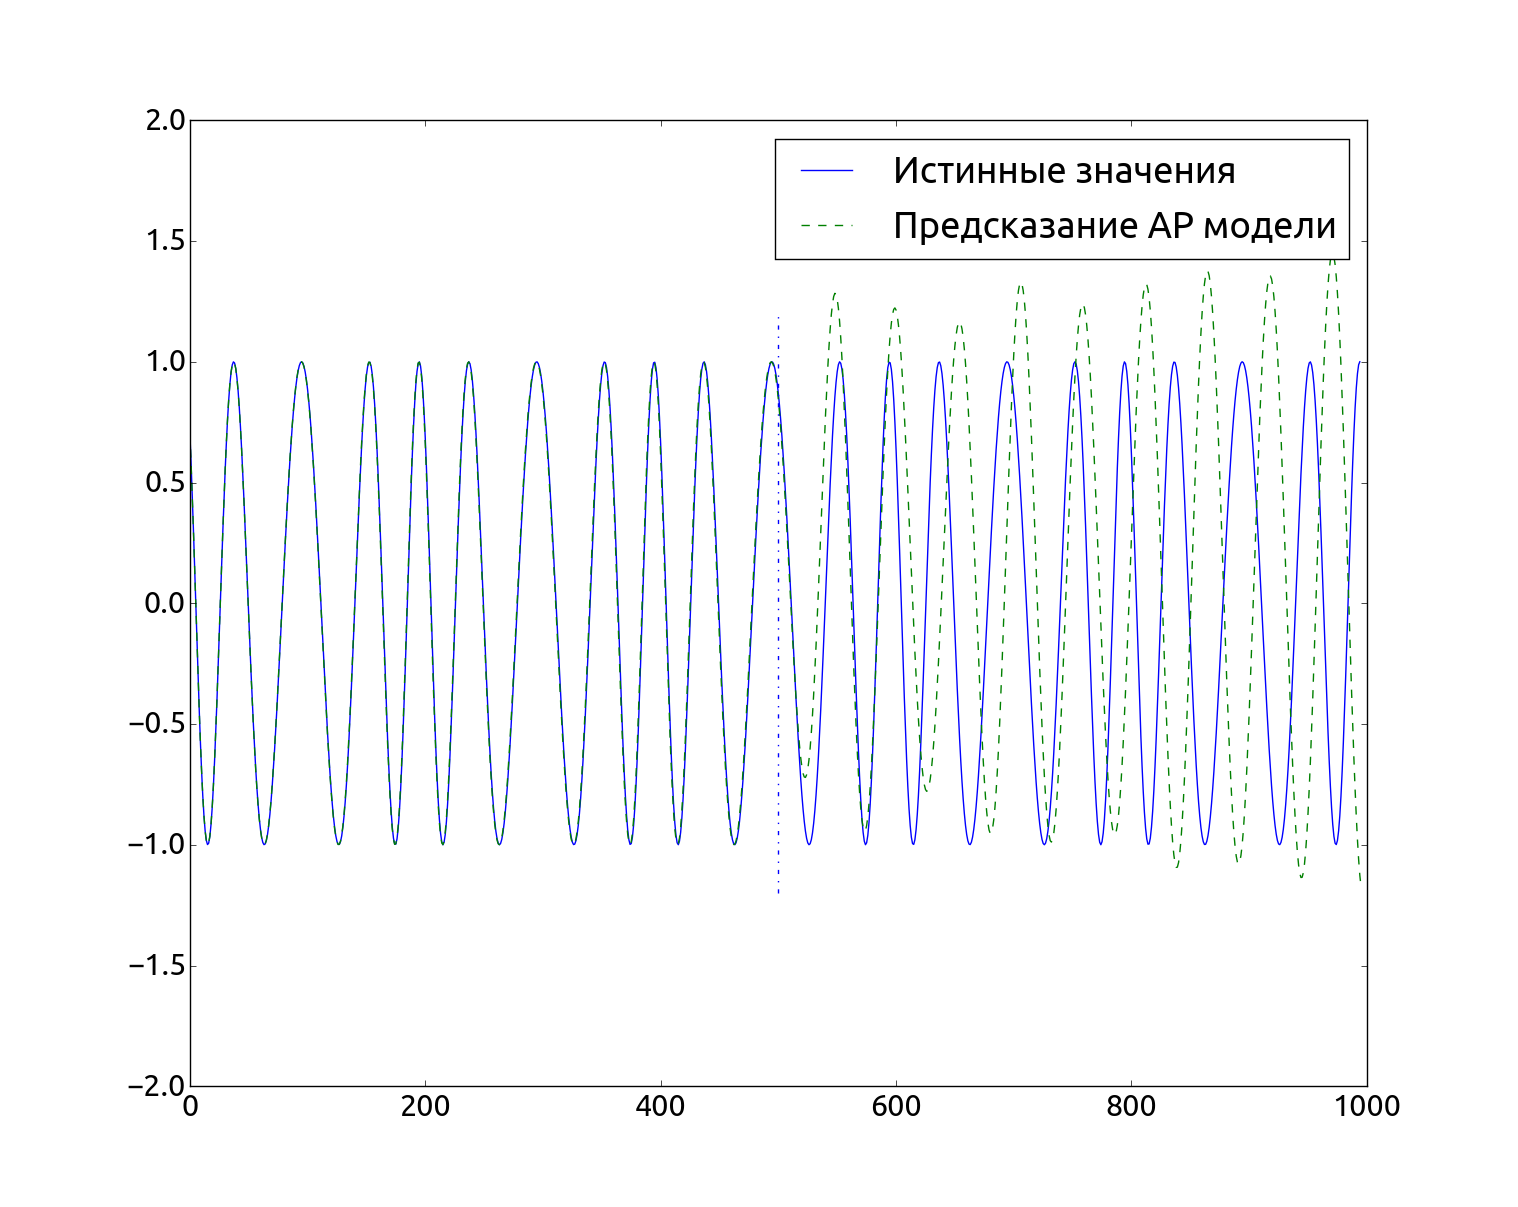
\includegraphics[width=0.9\textwidth]{theory/ar_pred_all}
  \caption{Предсказания $\AR$ модели на основе ранее предсказанных ей значений. Вертикальная линия отмечает начало модельных данных.}
  \label{fig:theory:ar_pred_all}
\end{figure}


\subsection{Модель скользящего среднего}

Авторегрессионная модель непосредственно учитывает абсолютные значения предыдущих наблюдений. Но когда они содержат шум, $\AR$ не может отделить его от сигнала и использует его наравне с полезной информацией. Из-за этого модель становится неустойчивой и качество приближения сильно ухудшается. Для описания шумовых процессов лучше подходит модель скользящего среднего (Moving Average model, $\MA$) (\autoref{eq:theory:ma}).

\begin{equation}
  \label{eq:theory:ma}
  X_t = \mu + \varepsilon_t + \sum_{i=1}^q \theta_i \varepsilon_{t-i}
\end{equation}
\begin{explanation}
\item[где] $\mu$ --- константа;
\item $\theta_1, \dotsc, \theta_q$ --- параметры модели;
\item $\varepsilon_t$ --- отклонение в момент времени $t$.
\end{explanation}

Она предполагает, что каждое следующее значение временного ряда выражается линейной комбинацией ошибок предсказаний на предыдущих шагах. Количество параметров называется порядком модели. Модель скользящего среднего $q$-го порядка обозначается $\MA(q)$.

\begin{figure}[h]
  \centering
  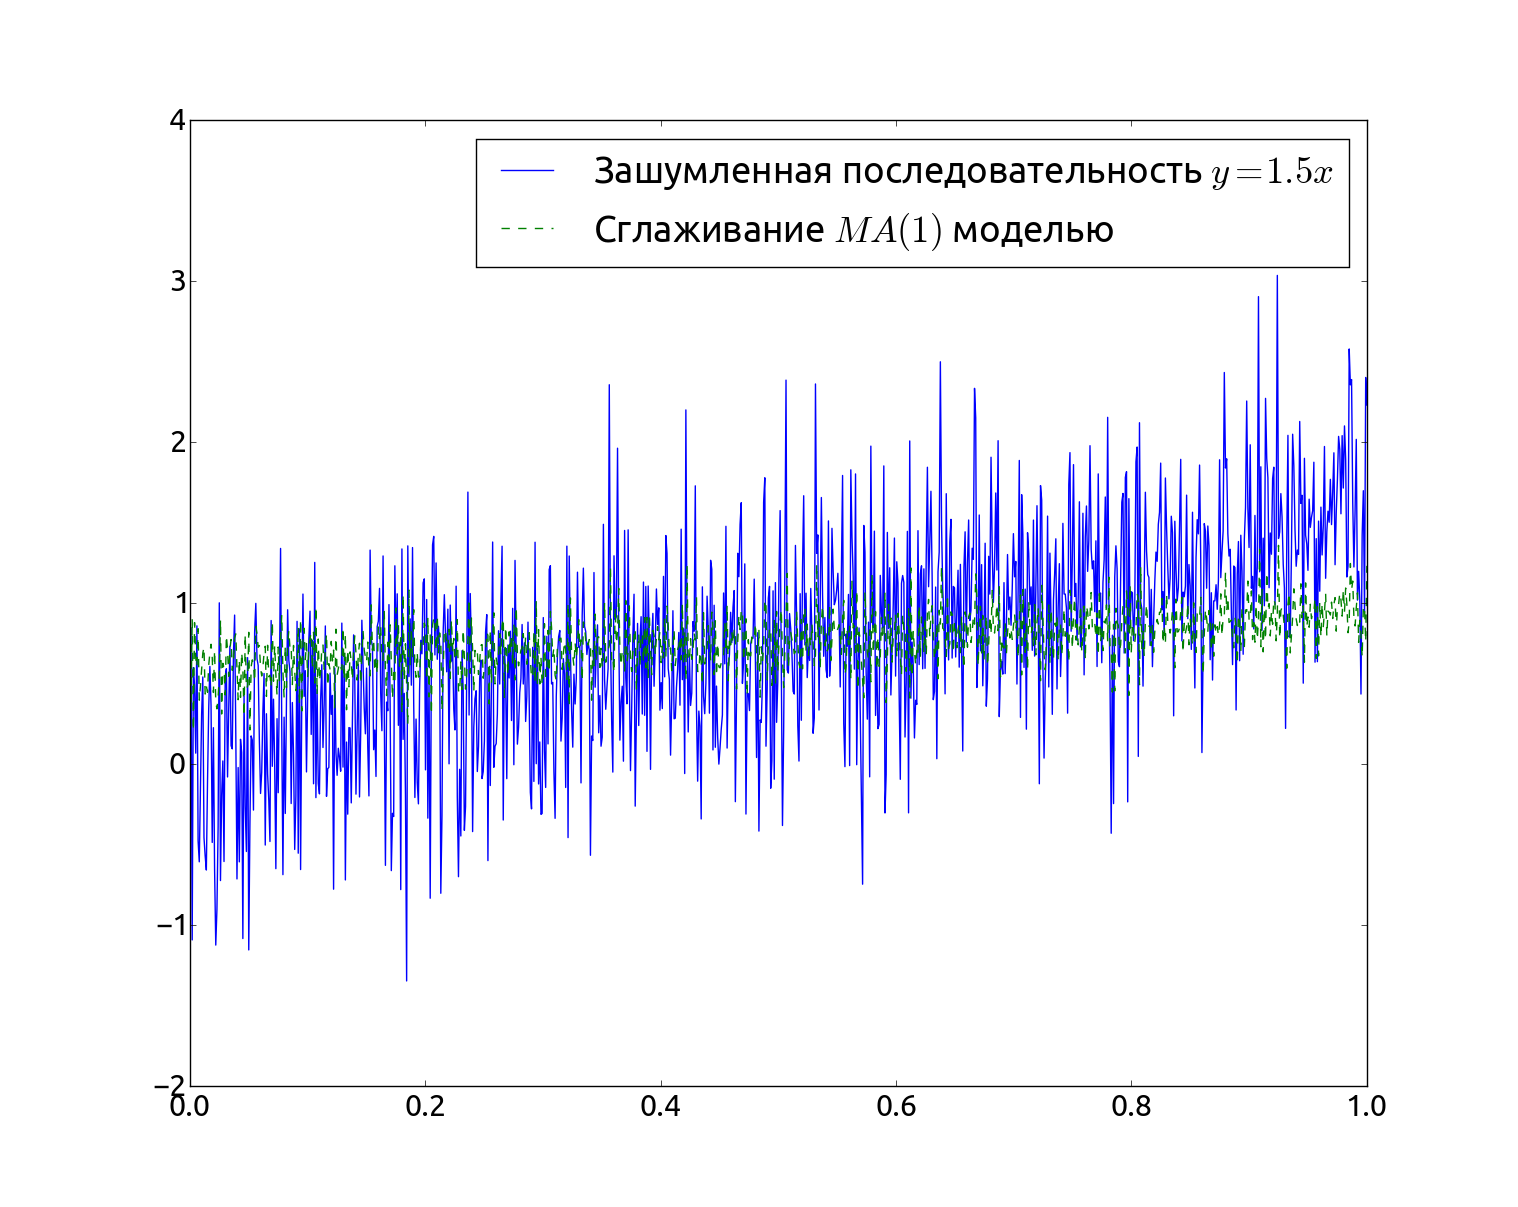
\includegraphics[width=0.9\textwidth]{theory/ma}
  \caption{Применение $\MA$}
  \label{fig:theory:ma}
\end{figure}

После перехода от абсолютных значений к относительным между $\AR$ и $\MA$ осталась некоторая связь. Всякий $\AR(p)$ процесс можно представить как $\MA(\infty)$. Покажем это на примере $\AR(1)$:

\begin{equation}
  \label{eq:theory:ar_as_ma}
  \begin{split}
    X_t & = \phi_1 X_{t-1} + \varepsilon_t \\
        & = \phi_1 (\phi_1 X_{t-2} + \varepsilon_{t-1}) + \varepsilon_t \\
        & = \phi_1 (\phi_1 (\phi_1 X_{t-3} + \varepsilon_{t-2}) + \varepsilon{t-1}) + \varepsilon_t \\
        & \dotso \\
        & = \varepsilon_t + \phi_1 \varepsilon_{t-1} + \phi_1^2 \varepsilon_{t-2} + \phi_1^3 \varepsilon_{t-3} + \dotsb
  \end{split}
\end{equation}

Получилась модель скользящего среднего бесконечно высокого порядка с коэффициентами $\theta_i = \phi_1^i$. Возможен и обратный переход. Это происходит благодаря общему принципу, на которых строятся два подхода --- линейная регрессия над данными из прошлого. Такой подход эффективен, когда нужно определить характеристики случайного процесса, а в наличии есть только его ряд наблюдаемых значений. Принципиально иные методы требуют больше информации, например, несколько коррелированных рядов.

Хотя мы увидели прямую связь между $\AR$ и $\MA$, на практике они обладают разным поведением и применяются для моделирования разных случайных процессов. Так получается, потому что в реальных задачах обычно используются модели невысоких порядков, тогда они имеют разные свойства.

Модель скользящего среднего используется для учета шума во временных рядах. Его невозможно предсказать, но нужно как-то обрабатывать, чтобы он не влиял на работу других моделей. Конечно, полностью избавится от него не удается, но получается уменьшить дисперсию, которую он привносит в процесс.

Как понятно из ее свойств, $\MA$ обычно не применяется сама по себе, а служит для предобработки данных, или как составная часть более сложных систем. Правильная композиция алгоритмов зачастую работает лучше, чем каждая ее составляющая.


\subsection{Модель авторегрессии --- скользящего среднего}

Зная достоинства и недостатки моделей авторегрессии и скользящего среднего, можно заметить, что они взаимодополняют друг друга. Первая неплохо настраивается под параметры случайного процесса, но неустойчива к шуму. Вторая плохо предсказывает сигнал, но сглаживает шумы. Идея их совмещения порождает качественно иную систему, называемую модель авторегрессии --- скользящего среднего ($\ARMA$).

\begin{equation}
  \label{eq:theory:arma}
  X_t = c + \varepsilon_t + \sum_{i=1}^p \phi_i X_{t-i} + \sum_{i=1}^q \theta_i \varepsilon_{t-i}
\end{equation}
\begin{explanation}
\item[где] $c$ --- константа;
\item $\varepsilon_t$ --- отклонение в момент времени $t$;
\item $\phi_1, \dotsc, \phi_p$ --- параметры авторегрессии;
\item $\theta_1, \dotsc, \theta_q$ --- параметры скользящего среднего.
\end{explanation}

Формула для $\ARMA$ представляет собой сумму составляющих ее моделей. Получается, каждое значение $X_t$ частично объясняется $\AR$ и частично $\MA$. В идеальном случае первая модель настраивается на полезную информацию, а вторая на шумовые отклонения.

Теперь в уравнении присутствуют и $p$, и $q$, поэтому появляется проблема выбора параметров и их балансировки. Во первых, высокие порядки улучшают качество подгонки под ряд, но ослабляют предсказательную силу модели. Во вторых, не всякая комбинация $p$ и $q$ дает рабочую модель. В процессе настройки параметров многократно решаются задачи оптимизации, а они имеют ограничения относительно своей целевой функции. Часто можно подобрать ряд, на котором эти ограничения не выполняются при заданном порядке модели и обучение модели становится невозможным. Это осложяет применение $\ARMA$ в автоматическом режиме, когда нужно анализировать много совершенно случайных процессов с совершенно различными характеристиками.

\begin{figure}[h]
  \centering
  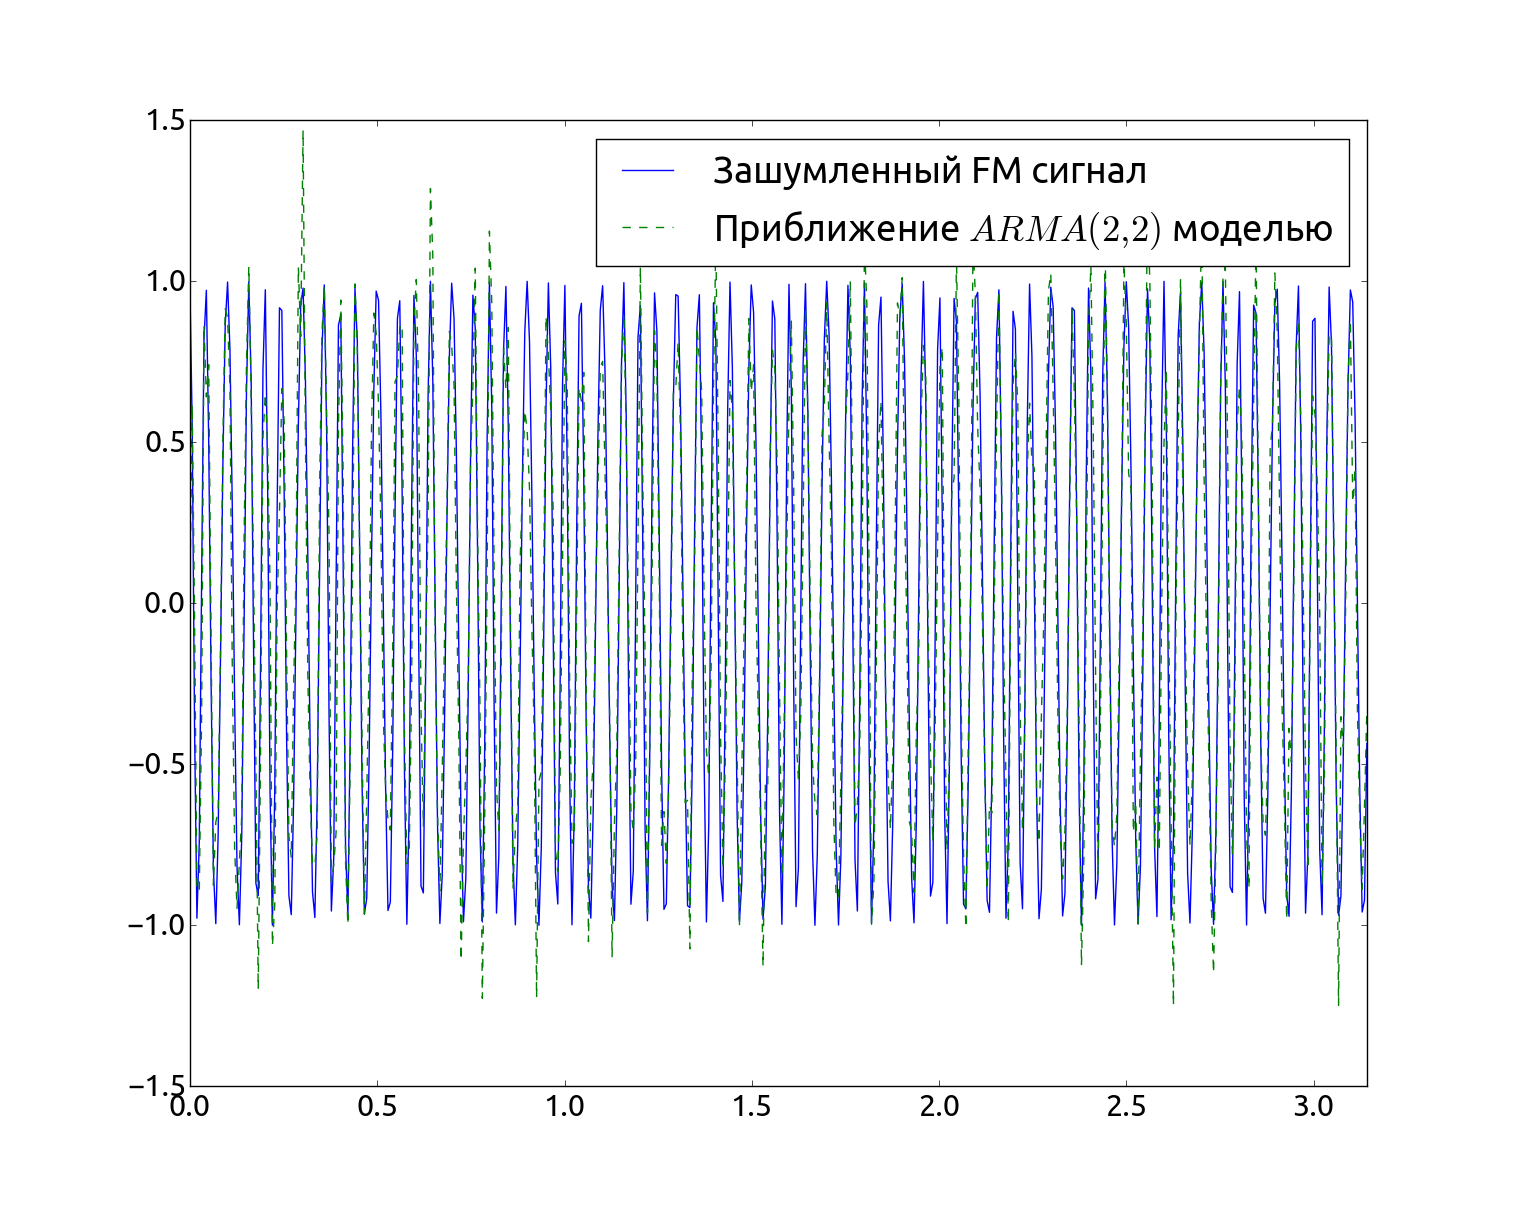
\includegraphics[width=0.9\textwidth]{theory/arma_modelled_fm}
  \caption{Настройка $\ARMA$ под модельный зашумленный FM сигнал}
  \label{fig:theory:arma_modelled_fm}
\end{figure}

На рисунке \ref{fig:theory:arma_modelled_fm} показано, как удается приблизить искусственный FM сигнал, содержащий шум. Видно, что модели не удается угадать точное значение амплитуды и она часто не добирает или выскакивает за реальные значения. Тем не менее, частота приближается достаточно точно, а именно мгновенная частота является определяющей характеристикой FM сигнала. Поэтому, можно сказать, что модель получилась неплохой. Важно заметить, что она настроилась на закономерности, лежащие в основе исходных данных и оказалась слабо подвержена влиянию шума.

\begin{figure}[h]
  \centering
  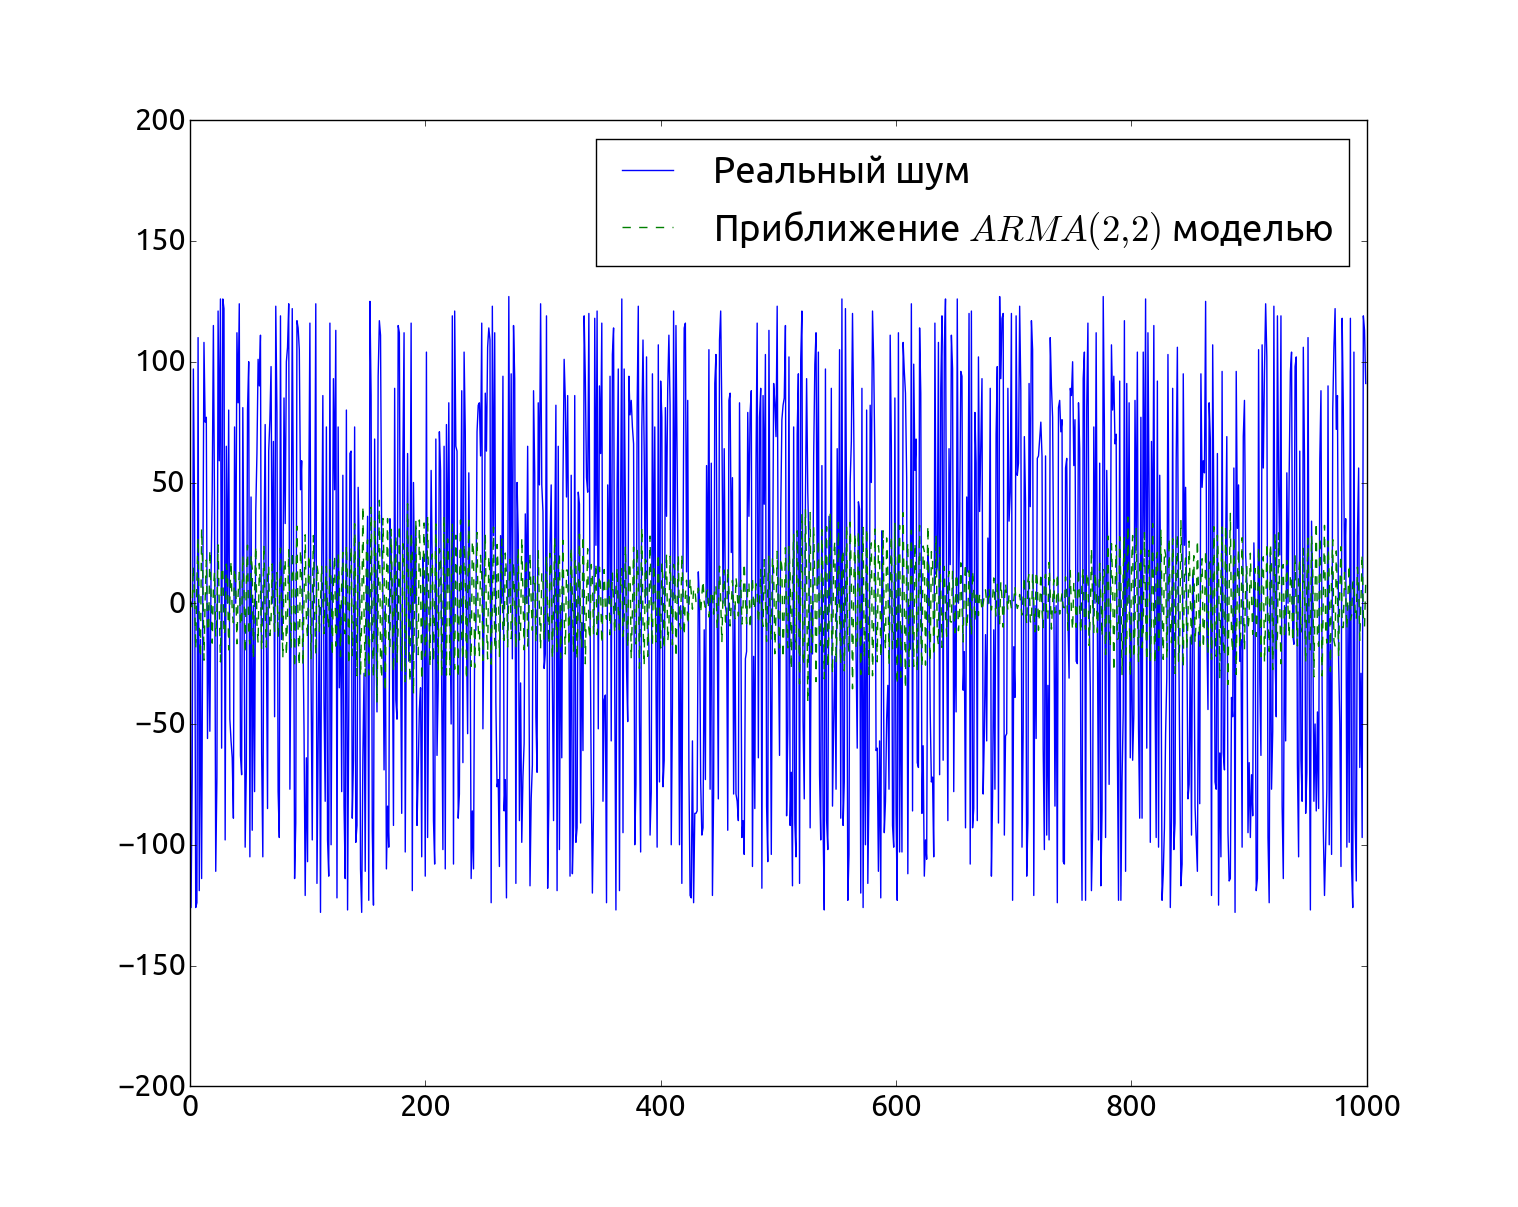
\includegraphics[width=0.9\textwidth]{theory/arma_real_noise}
  \caption{Настройка $\ARMA$ под реальный шум}
  \label{fig:theory:arma_real_noise}
\end{figure}

Для сравнения, на рисунке \ref{fig:theory:arma_real_noise} изображена модель с такими же параметрами, но настроенная на случайный шум. Она уже не приближается к максимальным значениям амплитуды, а колеблется ближе к нулю. Значит, в предсказании больший вес имеет модель скользящего среднего, а для авторегресии не удалось подобрать хороших параметров, поэтому ее влияние было ослаблено. В сравнении этих примеров хорошо видно очень полезное свойство $\ARMA$ --- автоматическое определение параметров приближаемого процесса и гибкая настройка под них. Если в данных есть какой-то сигнал и модель имеет достаточно высокий порядок, то она сумеет подстроиться под него, иначе будет стараться минимизировать ошибку, не отклоняясь далеко от среднего значения.

Этот алгоритм и его модификации нашли широкое применение в эконометрике. Его используют, если временной ряд интерпретируется как случайный процесс, обладающий постоянными на коротком интервале времени параметрами ($\AR$ часть), и испытывающий влияние внешних факторов, не доступных для непосредственного наблюдения ($\MA$ часть). Для этой задачи важна точность предсказания значений ряда в будущем и адаптивность под влияние внешних факторов.

В целях обнаружения сигналов предсказанное значение само по себе не несет полезной информации. Интересно рассмотреть использование $\ARMA$ для различения шумовых и не шумовых сигналов. Можно предположить, что достоверно предсказать информативный сигнал не получится --- для передачи информации нужно часто изменять параметры временного ряда, а модель хорошо работает на слабо стационарных рядах. Следовательно, на не шумовых сигналах ошибка приближения будет велика. Конечно, она будет велика и на случайном шуме, но не всякий шум случаен. Индустриальные помехи могут представлять собой постоянные колебания со слабо меняющейся частотой и мощностью. Эта особенность приближает их к слабо стационарному случайному процессу, который хорошо описывается моделью $\ARMA$. Значит, ее можно применять как фильтр некоторых индустриальных помех, которые по мощности и диапазону частот могут быть похожи на сигнал.

Другое ее применение, о котором уже упоминалось --- обнаружение разладок. Если в полосе частот работают радиосредства, иногда их можно заметить только в период активной передачи информации. В остальное время можно наблюдать только шум, или контрольный сигнал, который бывает сложно отличить от индустриальных помех. В этом случае можно настроить $\ARMA$ на наблюдаемый не информативный ряд. Тогда на предсказанных значения будет более или менее стабильная погрешность. Это говорит о том, что случайный процесс остается неизменным. Если же вдруг наблюдается резкий кратковременный скачок погрешности, это дает повод думать, что по каналу произошла передача информации. Продолжительный анализ повышает достоверность обнаружения. Дополнительным преимуществом метода является низкая вычислительная сложность --- модель достаточно построить один раз, после чего можно осуществлять предсказания по формуле \ref{eq:theory:arma}.

Из-за своей распространенности, методы работы с $\ARMA$ и ее компонентами эффективно реализованы в математических пакетах многих языков программирования. Часто они включают и процедуры выбора оптимального порядка модели. Это позволяет использовать даже в тех алгоритмах, где они играют лишь вспомогательную роль фильтрации или предобработки данных.
